%%This is a very basic article template.
%%There is just one section and two subsections.
\documentclass[a4paper, ngerman]{scrartcl}

\usepackage[T1]{fontenc}
\usepackage[utf8]{inputenc}
\usepackage[ngerman]{babel}
\usepackage{lmodern}
\usepackage{amsmath}
\usepackage{amsfonts}
\usepackage{hyperref}
\usepackage{graphicx}
\usepackage{paralist}


\hypersetup{
pdfborder = {0 0 0},
urlbordercolor = {0 0 0},
colorlinks = true,
linkcolor = black,
citecolor = black,
filecolor = black,
urlcolor  = black
}

\title{Software Challenge 2013 - Cartagena}
\subtitle{Spielregeln}



%% Variablen
\newcommand{\SpielSegmenteAnzahl}{\emph{5}}
\newcommand{\KartenAnzahl}{\emph{KartenAnzahl}}
\newcommand{\PiratenAnzahl}{\emph{6}}
\newcommand{\EmptyPlainPage}{\newpage\thispagestyle{plain}\ \newpage}
\newcommand{\RundenAnzahl}{\emph{30}}

\begin{document}
\maketitle

\begin{figure}[h]
	\centering
	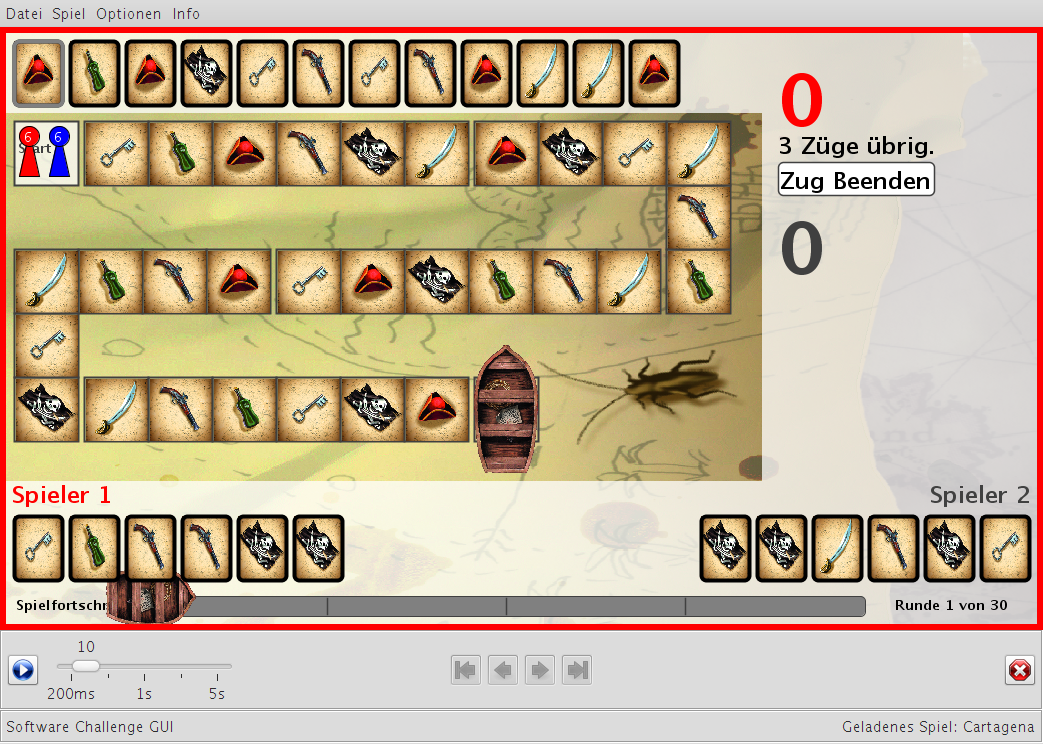
\includegraphics[width=\linewidth]{bilder/Uebersicht.png}
\end{figure}

"Die Nutzung des Spielkonzeptes "Cartagena" (Name, Spielregeln und Grafik)
erfolgt mit freundlicher Genehmigung der Winning Moves Deutschland GmbH."
\newpage
\tableofcontents
\newpage

\section{Einführung}
In dieser Anleitung werden die Elemente und Regeln des Spiels \emph{Cartagena}
der Soft\-ware\-challenge 2013 erläutert.\\
In dem Spiel versuchen zwei Spieler,
abwechselnd ihre Spielsteine, die Piraten, durch einen Tunnel zu bewegen.
Ziel des Spiels ist es, alle Piraten auf die Schaluppe zu bringen. Wer dies als
Erstes schafft, gewinnt das Spiel.\\
In der implementierten Version sind jedem Spieler die nächsten 12 ziehbaren
Karten, seine eigenen, sowie die Karten des Gegners bekannt. Die
in einer Spieltaktik zu beachtenden Parameter werden dadurch um ein Vielfaches
erhöht.

\section{Spielmaterial}
	\subsection{Das Spielbrett}
	Das Spielbrett setzt sich aus \SpielSegmenteAnzahl\ Segmenten zusammen,
	innerhalb derer die Symbole \emph{Schlüssel}, \emph{Flasche}, \emph{Hut},
	\emph{Pistole}, \emph{Flagge} und \emph{Säbel} jeweils genau einmal vorkommen.
	Die Reihenfolge ist innerhalb jedes Segmentes und von Spiel zu Spiel zufällig.
	Das Spielbrett wird durch ein Start- und ein Zielfeld ergänzt.
	Auf einem einzelnen Spielfeld dürfen, mit Ausnahme von Start- und Zielfeld
	jeweils maximal 3 Spielfiguren stehen.
	\subsection{Die Spielsteine}
	Jeder Spieler startet mit \PiratenAnzahl\ Piraten im Startfeld, welche alle ins
	Ziel gebracht werden müssen. Steht auf einem mehr als ein Pirat, so wird dies
	durch die Zahl im Kopf der Spielfigur angezeigt.
	\begin{figure}[h]
		\label{fig:Spielfeld}
		\centering
		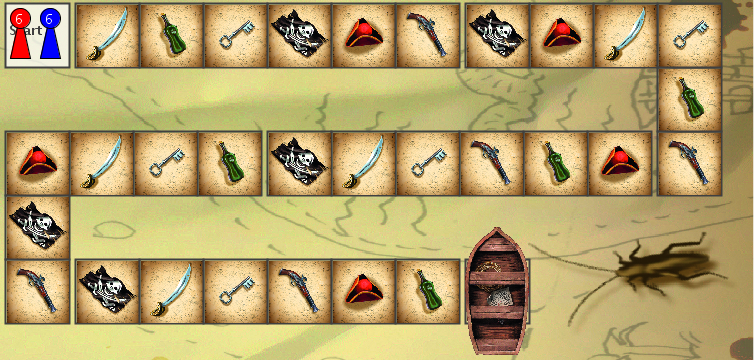
\includegraphics[scale = 0.5]{bilder/Spielfeld}
		\caption{Ein mögliches Spielfeld.}
	\end{figure}
	
	\subsection{Die Spielkarten}
	
	\begin{figure}[h]
		\centering
		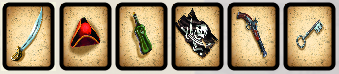
\includegraphics[scale = 0.5]{bilder/Karten}
		\caption{Die Spielkarten mit Symbolen}
	\end{figure}
	Zum Ziehen der Piraten werden die Spielkarten benötigt. Die Karten tragen
	analog zu den Spielfeldern wieder die Symbole \emph{Schlüssel}, \emph{Flasche}, \emph{Hut},
	\emph{Pistole}, \emph{Flagge} und \emph{Säbel}.\\
	Insgesamt gibt es 102 Karten, also 17 von jedem Symbol. Jeder Spieler startet
	mit 6 Karten auf der Hand und darf maximal 8 Karten auf der Hand halten.\\
	In der oberen Leiste werden die 12 Karten angezeigt, welche als
	nächstes gezogen werden können. Die Reihenfolge geht von links nach rechts.\\
	Sind alle Karten verbraucht, so werden die Karten vom Ablagestapel gemischt und
	neu bereitgelegt.
\section{Spielablauf}
	Es beginnt der rote Spieler. Jeder Spieler darf innerhalb einer Runde 3
	Teilzüge machen. Die Menge der Teilzüge darf aus einer beliebigen Kombination
	von Vorwärts- und Rückwärtszügen bestehen. Ein Spieler muss jedoch nicht alle 3
	Züge nutzen, kann also auch zwei, einen oder gar keinen Zug tätigen.\\
	Bei einem Vorwärtszug muss eine Karte von der Spielerhand abgelegt werden, bei
	Rückwärtszügen können neue Karten vom Stapel gezogen werden.
	
	\begin{figure}[h!]
		\label{fig:PossibleMoves}
		\centering
		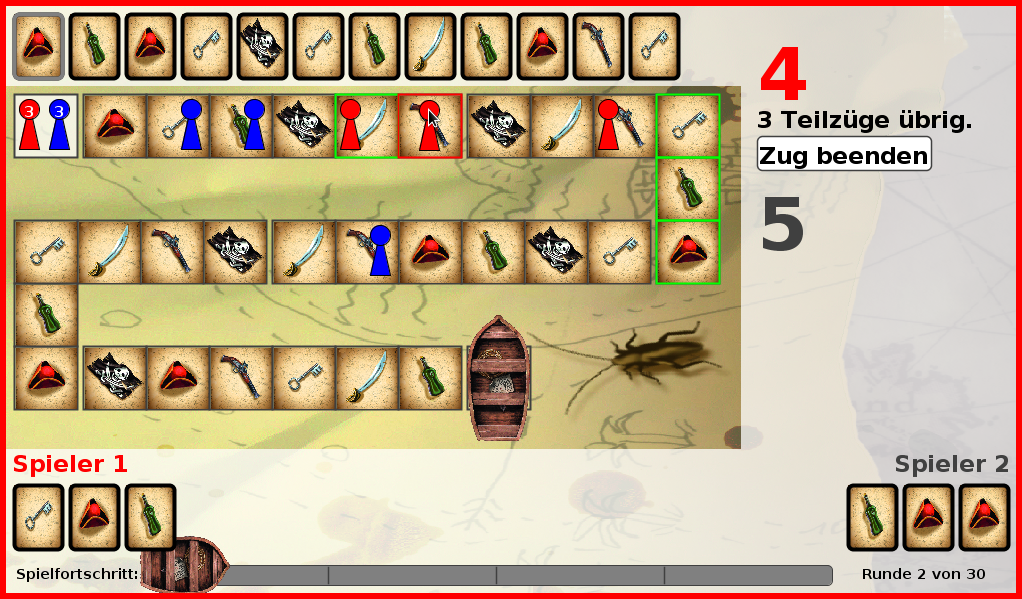
\includegraphics[scale = 0.5]{bilder/Moves}
		\caption{Eine Spielsituation, in der sowohl Vorwärts- als auch Rückwärtszüge
		möglich sind.}
	\end{figure}
	
	\subsection{Vorwärtszüge}
	Bei einem Vorwärtszug wählt ein Spieler ein Feld, auf dem sich mindestens eine 
	Spiel\-figur der eigenen Farbe befindet. Zum Vorwärtsziehen muss eine Karte
	abegelegt werden und die Spielfigur zieht auf das nächste unbesetzte Feld,
	welches das gleiche Symbol wie die Karte zeigt. Alle übrigen Felder sowie
	einfach oder mehrfach besetzte Felder werden hierbei übersprungen.\\
	Gibt es zwischen einem Piraten und der Schaluppe kein Feld mehr mit dem auf
	einer Karte abgebildeten Symbol oder sind alle Felder mit diesem Symbol
	belegt, so kann durch Ablegen dieser Karte direkt auf das Zielfeld gezogen
	werden.
	\begin{figure}[h]
		\centering
		\label{fig:Zielfeld}
		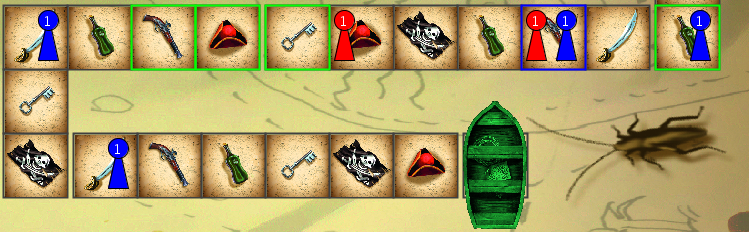
\includegraphics[scale = 0.5]{bilder/zielfeld}
		\caption{Alle Säbelfelder sind belegt und der blaue Spieler besitzt eine
		Säbelkarte.
		Durch Ablegen dieser Karte kann ins Zielfeld gezogen werden.}
	\end{figure}
	
	\subsection{Rückwärtszüge}
	Durch Rückwärtszüge können neue Karten von den offen liegenden Karten
	gezogen werden.
	Hierbei wählt ein Spieler eine Spielfigur aus und zieht sie auf das nächste
	zurückliegende Feld, auf dem bereits entweder eine oder zwei Spielfiguren
	stehen. Das Startfeld ist hierbei ausgeschlossen und es ist egal, welche Farbe
	die Spielsteine auf dem zurückliegenden Feld haben.\\
	Stehen auf dem zurückliegenden Feld 2 Piraten, so zieht der Spieler 2 neue
	Karten, sonst darf er nur eine Karte ziehen.
	
	\subsection{Punkteverteilung}
	Die Punkte ergeben sich aus der Anzahl der Piraten, welche sich im jeweiligen
	Segment befinden. Hat ein Spieler beispielsweise zwei Piraten in Segment 1 und
	einen Piraten in Segment 3, so ergibt sich eine Gesamtpunktzahl von 5.\\
	Spielsteine auf dem Startfeld bringen keine Punkte und ein Pirate im Zielfeld
	bringt 6 Punkte.
	
\section{Ende des Spiels}
	Hat ein Spieler alle seine Piraten im Zielfeld, so gewinnt dieser. Schafft dies
	keiner der beiden Spieler innerhalb der \RundenAnzahl\ Runden, so
	gewinnt der Spieler mit den meisten Punkten.
	
\section{Die graphische Benutzeroberfläche}
\subsection{Übersicht der graphischen Benutzeroberfläche}
	In Abbildung \ref{fig:GUI} ist ein Überblick der graphischen Benutzeroberfläche
	zu sehen. Die markanten Spielelemente sind mit \emph{a-e} gekenzeichnet.
	 \begin{figure}[h!]
		\centering
		\label{fig:GUI}
		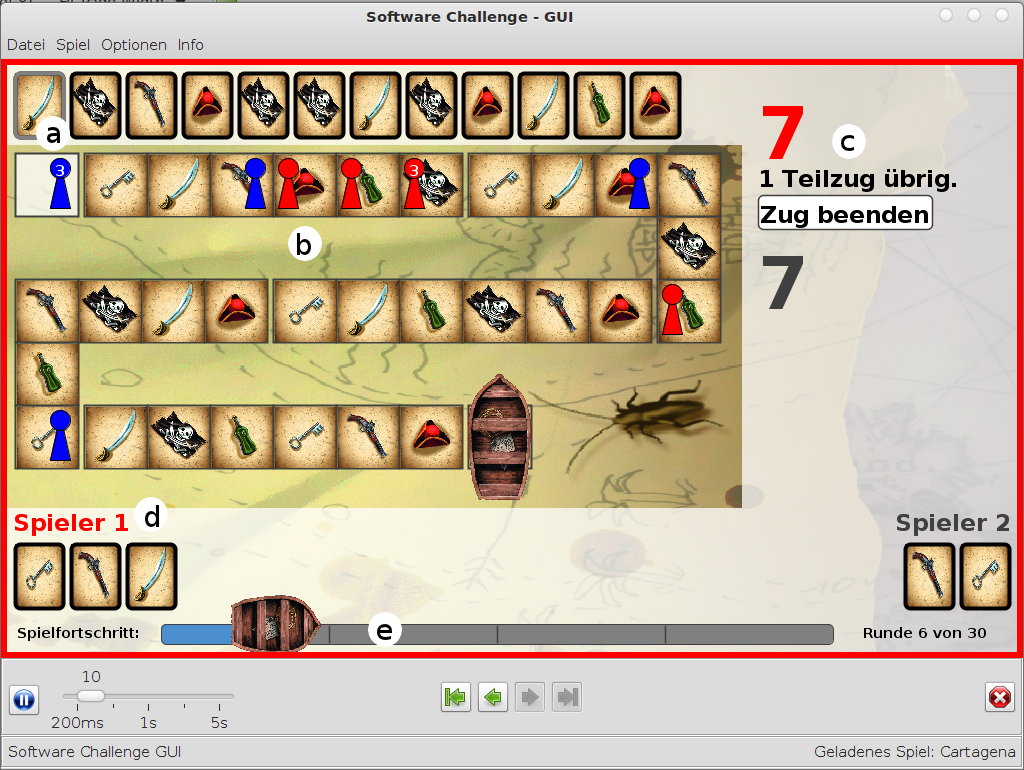
\includegraphics[width=\linewidth]{bilder/gui}
		\caption{Überblick der GUI}
	\end{figure}
	
	\begin{compactenum}[a)]
		\item Die nächsten ziehbaren Karten. Die erste befindet sich links.
		\item Das Spielbrett
		\item Punkteanzeige, Anzeige der verbleibenden Züge und Button um einen Zug
		vorzeitig zu beenden. Die Punkte des roten Spielers sind oben, die des blauen
		Spielers unten.
		\item Die Karten, welche Spieler 1 auf der Hand hält.
		\item Spielfortschrittsanzeige
	\end{compactenum}
	
\subsection{Das Einstellungsmenü}
	 \begin{figure}[h]
		\centering
		\label{fig:Configuration}
		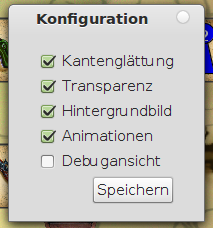
\includegraphics[scale=0.5]{bilder/configuration}
		\caption{Das Einstellungsmenü}
	\end{figure}
	
	Ein Einstellungsmenü mit Darstellungsoptionen lässt
sich über die Leertaste anzeigen. Dazu muss das
Spielfeld den Tastaturfokus haben (erforderlichenfalls
vorher Mausklick auf das Spielfeld). Es stehen dort
folgende Einstellungen zur Verfügung:

\textbf{Kantenglättung} und \textbf{Transparenz} verbessern die
Optik des Spiels, sind aber rechenintensiv. Auf sehr
langsamen Rechnern sollten sie daher deaktiviert
werden. \textbf{Hintergrundbild} ist zwar weniger rechenintensiv, kann
aber auch aus Gründen der Übersichtlichkeit deaktiviert
werden.\\
\textbf{Animationen} legt fest, ob die Bewegungen der Spielsteine in Wiederholungen und bei Computerspielern
animiert werden sollen.\\
Die \textbf{Debugansicht} verkleinert die Punkteanzeige in
der Seitenleiste etwas und zeigt unterhalb Debug
Hilfestellungen zu einzelnen Zügen an. Diese Hilfestellungen sind Texte, die ein Spielclient einem Zug
beifügen kann, den er an den Spielserver sendet.
	
\end{document}
